%!TEX encoding = UTF-8 Unicode
%
% Laboratorio di Fisica III
% Esperienza 11
% Anno accademico 2013/2014
% Daniele Brugnara, Alessandro Casalino
%

\documentclass {article}
\usepackage[utf8]{inputenc}
\usepackage{fontenc}
\usepackage[english]{babel}
\usepackage[%hypertex,
                 unicode=true,
                 plainpages = false, 
                 pdfpagelabels, 
                 bookmarks=true,
                 bookmarksnumbered=true,
                 bookmarksopen=true,
                 breaklinks=true,
                 backref=false,
                 colorlinks=true,
                 linkcolor = blue,		% Use "blue" if you want to highlight them
                 urlcolor  = blue,
                 citecolor = red,
                 anchorcolor = green,
                 hyperindex = true,
                 linktocpage = true,
                 hyperfigures
]{hyperref}
\usepackage{graphicx}
\usepackage{float}
\usepackage{fancyhdr}
\usepackage{listingsutf8}
\usepackage{xcolor}
\graphicspath{{figures/PNG/}{figures/PDF/}{figures/}}
\usepackage{amsfonts}
\usepackage{amsmath}
\usepackage{amssymb}	
\usepackage{wrapfig}
\usepackage{enumitem}
\usepackage{subfigure}
\usepackage{amssymb}
\usepackage{amsmath}
\usepackage [a4paper, top=2.5cm, bottom=2cm, left=1.5cm, right=1.5cm] {geometry}
\pagestyle{fancy}

% cambiato bottom da 1.8 + logo

\makeatletter
\@addtoreset{section}{part}
\makeatother
\rhead{\LARGE Project 1}

\lhead{\large Numerically solving a differential equation}
\lfoot{D. Brugnara, M. Seclì}
\cfoot{}
\rfoot{\thepage}
\renewcommand{\headrulewidth}{0.7pt}
\renewcommand{\footrulewidth}{0.7pt}

\definecolor{dkgreen}{rgb}{0,0.6,0}
\definecolor{dred}{rgb}{0.545,0,0}
\definecolor{dblue}{rgb}{0,0,0.545}
\definecolor{lgrey}{rgb}{0.9,0.9,0.9}
\definecolor{gray}{rgb}{0.4,0.4,0.4}
\definecolor{darkblue}{rgb}{0.0,0.0,0.6}
\lstdefinelanguage{cpp}{
      backgroundcolor=\color{lgrey},  
      basicstyle=\footnotesize \ttfamily \color{black} \bfseries,   
      breakatwhitespace=false,       
      breaklines=true,               
      captionpos=b,                   
      commentstyle=\color{dkgreen},   
      deletekeywords={...},          
      escapeinside={\%*}{*)},                  
      frame=single,                  
      language=C++,                
      keywordstyle=\color{purple},  
      morekeywords={BRIEFDescriptorConfig,string,TiXmlNode,DetectorDescriptorConfigContainer,istringstream,cerr,exit}, 
      identifierstyle=\color{black},
      stringstyle=\color{blue},      
      numbers=right,                 
      numbersep=5pt,                  
      numberstyle=\tiny\color{black}, 
      rulecolor=\color{black},        
      showspaces=false,               
      showstringspaces=false,        
      showtabs=false,                
      stepnumber=1,                   
      tabsize=5,                     
      title=\lstname,                 
    }

\author{
%\textbf{\normalsize Gruppo A6:}\\
\normalsize Daniele Brugnara \texttt{$<$\href{mailto:daniebru@mail.uio.no}
{daniebru@mail.uio.no}$>$}\\
\normalsize Martina Cammilli \texttt{$<$\href{mailto:martinacam@mail.uio.no}
{martinacam@mail.uio.no}$>$}\\
\normalsize Matteo Seclì \texttt{$<$\href{mailto:mattes@mail.uio.no}
{mattes@mail.uio.no}$>$}
}
\title{\textbf{Project 1: numerically solving a differential equation through a linear system}}

\begin{document}

\maketitle

\hrule
%\medskip
\begin{center}
	\large\textbf{Abstract}
	\medskip\\
	\begin{minipage}[c][][c]{0.8\textwidth}
		\small{
			In this project we aim to solve a special kind of differential equation using a numerical procedure that allows us to express the equation through a linear system. We will study some algorithms to solve such a problem, focusing on the efficiency of the program, setting our goal more on speed than generality.
			}
	\end{minipage}
\end{center}
\medskip
\hrule

\section{Introduction}

The differential equation we're interested in studying is of the type

\begin{equation}
	u''(x)= - f(x)
	\label{differential_eq}
\end{equation}

In our case we will limit our solutions using the contour conditions of $u(0)=0$ and $u(L)=0$, where $[0, L]$ is our domain of integration.
Using Taylor expansion it is possible to express the second derivative of a function $u(x)$ as

\begin{equation}
	u''(x)= \frac{u(x-h)-2 u(x)+u(x+h)}{h^2}+ \O (h^2)
\end{equation}

We are therefore able to discretize equaition (\ref{differential_eq}) using $N$ points, obtaining:

$$u''_i= \frac{u_{i-1}-2 u_i+u_{i+1}}{h^2}=-f_i \quad \quad i \in \left\lbrace 1 \cdots N\right\rbrace$$

Using the matrix representation, we can write equation (\ref{differential_eq}) as

\begin{equation}
 \begin{pmatrix}
   2 & -1 &  0 & 0 & \cdots & 0  \\
  -1 &  2 & -1 & 0 & \cdots & 0  \\
   0 &-1 &  2 & -1 & \cdots & 0 \\
  \vdots  & \vdots  & & \ddots & & \vdots   \\
   0 &  0 & \cdots  & -1 & 2 & -1 \\
   0 &  0 & \cdots & \cdots  & -1 & 2
 \end{pmatrix}
 \begin{pmatrix}
  u_0 \\
  u_1 \\
  u_2 \\
  \vdots  \\
  u_{N-2} \\
  u_{N-1} 
 \end{pmatrix}
 = h^2
 \begin{pmatrix}
  f_0 \\
  f_1 \\
  f_2 \\
  \vdots  \\
  f_{N-2} \\
  f_{N-1} 
 \end{pmatrix}
\end{equation}

Note how, with this system it is already implied that $f(0)=0$ e $f(L)=0$, since the first and last equations state that

$$h^2 f_0=\frac{2 u_0-u_1}{h^2}=\frac{-1 u_{-1}+2 u_0-u_1}{h^2}$$

$$h^2 f_{N-1}=\frac{-u_{N-2}+2 u_{N-1}}{h^2}=\frac{-u_{N-2}+2 u_{N-1}-u_N}{h^2}$$ 

Since the boundary conditions of the differential equations state that $u_{-1}=u(0)=0$ and $u_{N}=u(L)=0$.  

This linear system is indeed very particular and has a clear pattern. We will first focus on finding a solving algorithm for a general tridiagonal matrix and after we will try to implement another program to solve this particular system with the intent of lowering the number of calculation and therefore the computation time.

\section{General algorithm for solving a tridiagonal matrix through back and forward substitution}

A general tridiagonal system can be expressed as

\begin{equation}
 \begin{pmatrix}
   b_0 & c_0 &  0 & 0 & \cdots & 0  \\
  a_1 & b_1 & c_1 & 0 & \cdots & 0  \\
   0 & a_2 &  b_2 & c_2 & \cdots & 0 \\
  \vdots  & \vdots  & & \ddots & & \vdots   \\
   0 &  0 & \cdots  & a_{N-2} & b_{N-2} & c_{N-2} \\
   0 &  0 & \cdots & \cdots  & a_{N-1} & b_{N-1}
 \end{pmatrix}
 \begin{pmatrix}
  u_0 \\
  u_1 \\
  u_2 \\
  \vdots  \\
  u_{N-2} \\
  u_{N-1} 
 \end{pmatrix}
 =h^2
 \begin{pmatrix}
  f_0 \\
  f_1 \\
  f_2 \\
  \vdots  \\
  f_{N-2} \\
  f_{N-1} 
 \end{pmatrix}
\end{equation}

We will describe the algorithm we used for this system first for a 3x3 tridiagonal matrix, and after we will demonstrare its validity for a square tridiagonal matrix of optional dimension.
\\
\\
\\
\\
\\
MATRIX 3X3:

\begin{equation}
\left(
\begin{array}{ccc|c}
   b & c &  0 & f_0 \\
   a & b &  c & f_1 \\
   0 & a &  b & f_2 \\
   \cdots  & \cdots  & \cdots \\
\end{array}	
\right)
\longrightarrow
\end{equation}
\begin{equation}
Passage 1:
\left(
\begin{array}{ccc|c}
   1 & c/b & 0 & f_0/b \\
   a & b & c & f_1 \\
   0 & a & b & f_2 \\
\end{array}
\right)
\longrightarrow\\
\end{equation}
\begin{equation}
Passage 2:
\left(
\begin{array}{ccc|c}
  1 & c/b & 0 & f_0/b \\
  0 & \frac{b-(c/b)a)}{b-(c/b)a} & \frac{c}{(b-(c/b)a} & \frac{f_1-af_0}{b-(c/b)a} \\
  0 & 0 & \frac{b-\frac{ac}{b-ac/b}}{b-\frac{ac}{b-ac/b}} & \frac{f_2-af_1}{b-\frac{ac}{b-ac/b}} \\ 
\end{array}
\right)
=
\left(
\begin{array}{ccc|c}
  1 & c/b & 0 & f_0/b \\
  0 & 1 & \frac{c}{b-ac/b} & \frac{f_1-af_0}{b-(c/b)a} \\
  0 & 0 & 1 & \frac{f_2-af_1}{b-\frac{ac}{b-ac/b}} \\ 
\end{array}
\right)
\longrightarrow\\\
\end{equation}
\begin{equation}
Passage 3:
\left(
\begin{array}{ccc|c}
  1 & 0 & 0 & f_0/b-f_1(c/b) \\
  0 & 1 & 0 & \frac{f_1-af_0}{b-(c/b)a}-f_2\frac{c}{b-ac/b} \\
  0 & 0 & 1 & \frac{f_2-af_1}{b-\frac{ac}{b-ac/b}} \\
\end{array}
\right)
\end{equation}

Now it's very simple to solve the system.
\\
\\
\\
MATRIX (n+1)x(n+1)

Before starting to demonstrate that the above passages can be done also for a (n+1)x(n+1) matrix, supposed that they work for a nxn one, we can notice that, in general, for a square matrix of optional dimension N, doing the passage 2 until the penultime row we obtain:

$$A_{N-1,N}=\frac{c}{bet(N-1)}$$
where 
$$bet(n)=b_0-\frac{ac}{b_1-\frac{ac}{b_2-\frac{ac}{\frac{\cdots}{b_{n-1}-\frac{ac}{b_n}}}}}$$
(here all the $b_i's$ have the same value; the index i helps only to count them).

Now we do the passage 2 until the last row (we focus only on the tridiagonal matrix; if we manage to obtain the unitary matrix the system is solved); we obtain:

\begin{equation}
\left(
\begin{array}{ccccc}
  1 & c/b & 0 & 0 & \cdots \\
  0 & 1 & fract{c}{b-ac/b} & 0 & \cdots \\
  \cdots & \cdots & \cdots & \cdots & \cdots \\
  \cdots & \cdots & \cdots & 1 & c/bet(n) \\
  \cdots & \cdots & \cdots & 0 & 1 \\
\end{array}
\right)
\end{equation}
and simply subtracting, from the n-row, the (n+1)-row multiplied for bet(n)/c:
\begin{equation}
\left(
\begin{array}{ccccc}
  1 & c/b & 0 & 0 & \cdots \\
  0 & 1 & \frac{c}{b-ac/b} & 0 & \cdots \\
  \cdots & \cdots & \cdots & \cdots & \cdots \\
  \cdots & \cdots & \cdots & 1 & 0 \\
  \cdots & \cdots & \cdots & 0 & 1 \\
\end{array}
\right)
\end{equation}

Now, ignoring the (n+1)-row and the (n+1)-column, we have a nxn matrix which we can bring back to the identity going on with the passage 3.
\\
\\
\\
ALGORITHM IN C++

Translating the above algorithm in C++ language and working only on the vector f and on the solution vector u, we obtain the following code:

\begin{lstlisting}[language=cpp]
	u[0]=f[0]/(bet=b);
    for(int j = 1; j < N; j++) {
        gam[j]=c/bet;
        bet=b-a*gam[j];
        u[j]=(f[j]-a*u[j-1])/bet;
    }
    for (int j = (N-2); j >= 0; j--) u[j] -= gam[j+1]*u[j+1];
\end{lstlisting}

\subsection{Particular algorithm}

Using the regular Gaussian elimination algorithm we proceed to find a specific solution of our system as follows:

\begin{equation}
\left(
\begin{array}{cccccc|c}
   2 & -1 &  0 & 0 & \cdots & 0 & f_0 \\
  -1 &  2 & -1 & 0 & \cdots & 0 & f_1 \\
   0 &-1 &  2 & -1 & \cdots & 0 & f_2\\
  \vdots  & \vdots  & & \ddots & & \vdots & \vdots  \\
   0 &  0 & \cdots  & -1 & 2 & -1 & f_{N-2} \\
   0 &  0 & \cdots & \cdots  & -1 & 2 & f_{N-1} 
\end{array}	
\right)
\longrightarrow
\left(
\begin{array}{cccccc|c}
   2 & -1 &  0 & 0 & \cdots & 0 & f_0 \\
   0 &  3 & -2 & 0 & \cdots & 0 & 2 f_1+f_0 \\
   0 & 0 &  4 & -3 & \cdots & 0 & 3 f_2+2 f_1+f_0\\
  \vdots  & \vdots  & & \ddots & & \vdots & \vdots  \\
   0 &  0 & \cdots  & 0 & N & -(N-1) &  (N-1) f_{N-2} + \sum_{j=0}^{N-3} (j+1)f_{j}  \\
   0 &  0 & \cdots & \cdots  & 0 & N+1 &  \sum_{j=0}^{N-1} (j+1)f_{j} 
\end{array}	
\right)
\end{equation}

We therefore know ahead of times the explicit form of the matrix in upper triangular form and are able to compute all the constant terms of the system as follows

$$\tilde{f}_i= \sum_{j=0}^{i}(j+1) f_j$$

However, we don't need to compute the sum every time, since we can compute $\tilde{f}_i$ knowing $\tilde{f}_{i-1}$:

$$\tilde{f}_i=(i+1)f_i+\tilde{f}_{i-1}$$

Once this forward computations are completed, it is possible to proceed with a back substitution, knowing that

$$u_{N-1}=\frac{1}{N+1} \tilde{f}_{N-1}$$

we are able to find the vector of solutions $u_i$

$$u_i=\frac{1}{i+2} (\tilde{f}[i]+ (i+1) u[i+1])$$

Translating the algorithm in C++ code we obtain the following cycle:

\begin{lstlisting}[language=cpp]
	for (i=1; i!=n; i++) {
		f[i]=(i+1)*f[i]+f[i-1];
	}
	u[n-1]=f[n-1]/(n+1);
	for (i=n-2; i>=0; i--) {
		u[i]=(f[i]+(i+1)*u[i+1])/(i+2);
	}
\end{lstlisting}

Similarly to the previous code of section 1.2 this algorithm is characterized by 2 for cycles and therefore the time required for the solution increase linearly with the number of points used.

Moreover, this program allows us to use a minimal amount of memory, storing only the vector f and the solution u. 

We will now prove by induction con the dimension of the matrix the validity of the algorithm. We will first prove it for a matrix of $3 \times 3$ dimension and then prove that given  





\section{Errors}
It is now interesting to analyse the error that we do in numerical approximation as a function of the number of points. It is intuitive that, as much as we restrict the step length $h$ (that is the same thing as increasing the number of points) the error gets smaller and smaller. This behaviour is shown if Figure \ref{fig:errors}, where we plotted in a log-log scale the maximum percentage error calculated as
\begin{equation*}
	\epsilon_i = \left| \frac{v[i]}{u[i]} - 1 \right|
\end{equation*}
($v[i]$ is the numerical solution, $u[i]$ is the analytical one).
\begin{figure}[H]
	\centering
	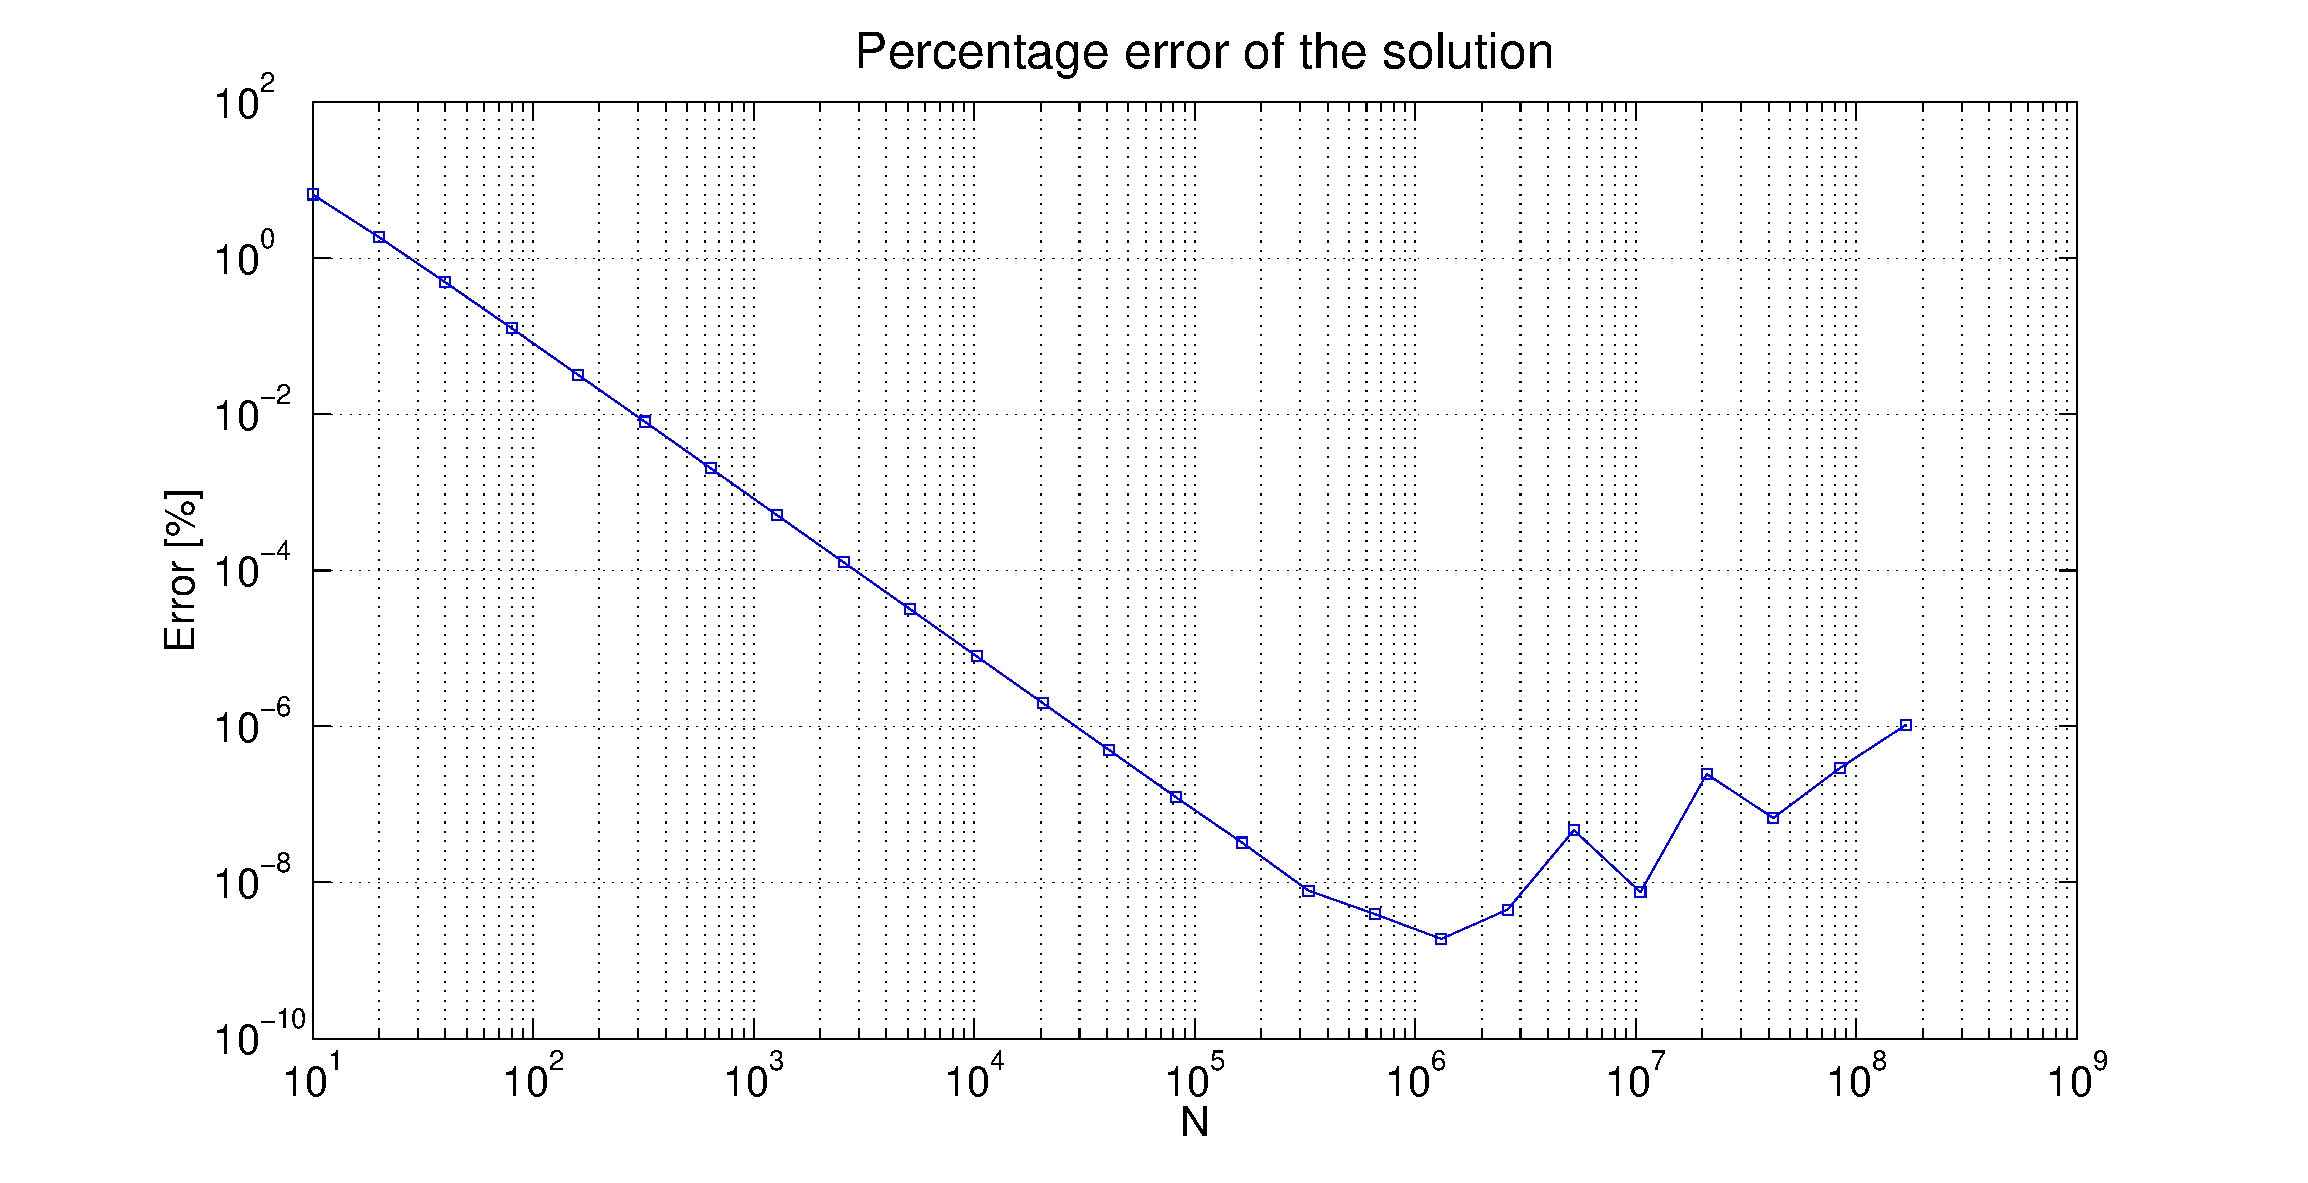
\includegraphics[width=\textwidth]{errors}
	\caption{Maximum percentage error of the numerical solution as a function of the number of points.}
	\label{fig:errors}
\end{figure} 
You see that the error lowers until $N = 10^{5}$, then increases again. This a typical example of \emph{loss of precision}; as our numerical solution gets closer to the analytical one, the ratio $v[i]/u[i]$ gets closer to one, and as a result in calculating $\epsilon_i$ we perform a subtraction between two almost identical (in our choice of precision) numbers. This causes a loss in terms of significant digits that explains the behaviour of the plot for big $N$. It is also evident that we get the lowest significant relative error for $N \simeq 10^{6}$. Relative errors for $N > 10^{6}$ are not worth trusting, due to the loss of precision explained above.


\end{document}